%
\chapter{Software Development Life Cycle Models}%\vspace{1cm}
Software development life cycle refers to the process of software development.
The standard for software life cycle processes, describes the development
process as consisting of requirements, design, code, and testing.
There are different approaches to break down the work when developing software
systems. Conceptually, each model provides specific guidance to the
sequencing and repetition of life cycle activities to deliver software systems.

\vspace{3mm}

There is no process that can fit all projects. The most important factors
to choose the best model are the following ones:
\begin{itemize}
\item Project Scope/Size
\item Organizational Cultutre
\item Involved People
\item Criticality
\item Stability
\end{itemize}

\ifslides
\\
\else
%\\[3ex]
\fi
%
%Wir betrachten hier die zwei wichtigsten Vertreter:
\begin{minipage}[t]{0.35\linewidth}
\section{Build and fix model}
no specific procedure
\begin{center}
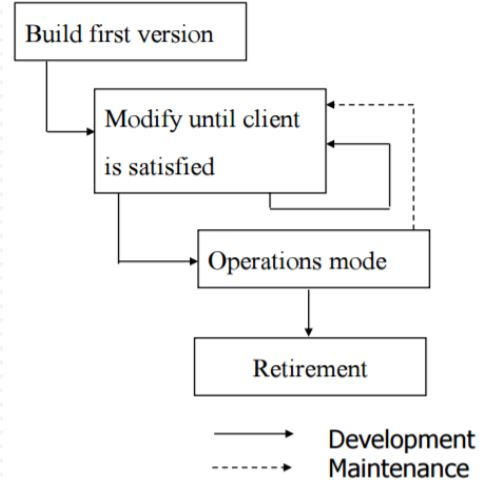
\includegraphics[width=\linewidth]{lifecycle/img/buildandfix.jpg}
\end{center}
\end{minipage}
\hfill
%
\ifslides
\begin{minipage}[t]{0.5\linewidth}
\else
\begin{minipage}[t]{0.5\linewidth}
\fi
\section{Waterfall model}
sequential, fixed, not adaptive
\begin{center}
\ifslides
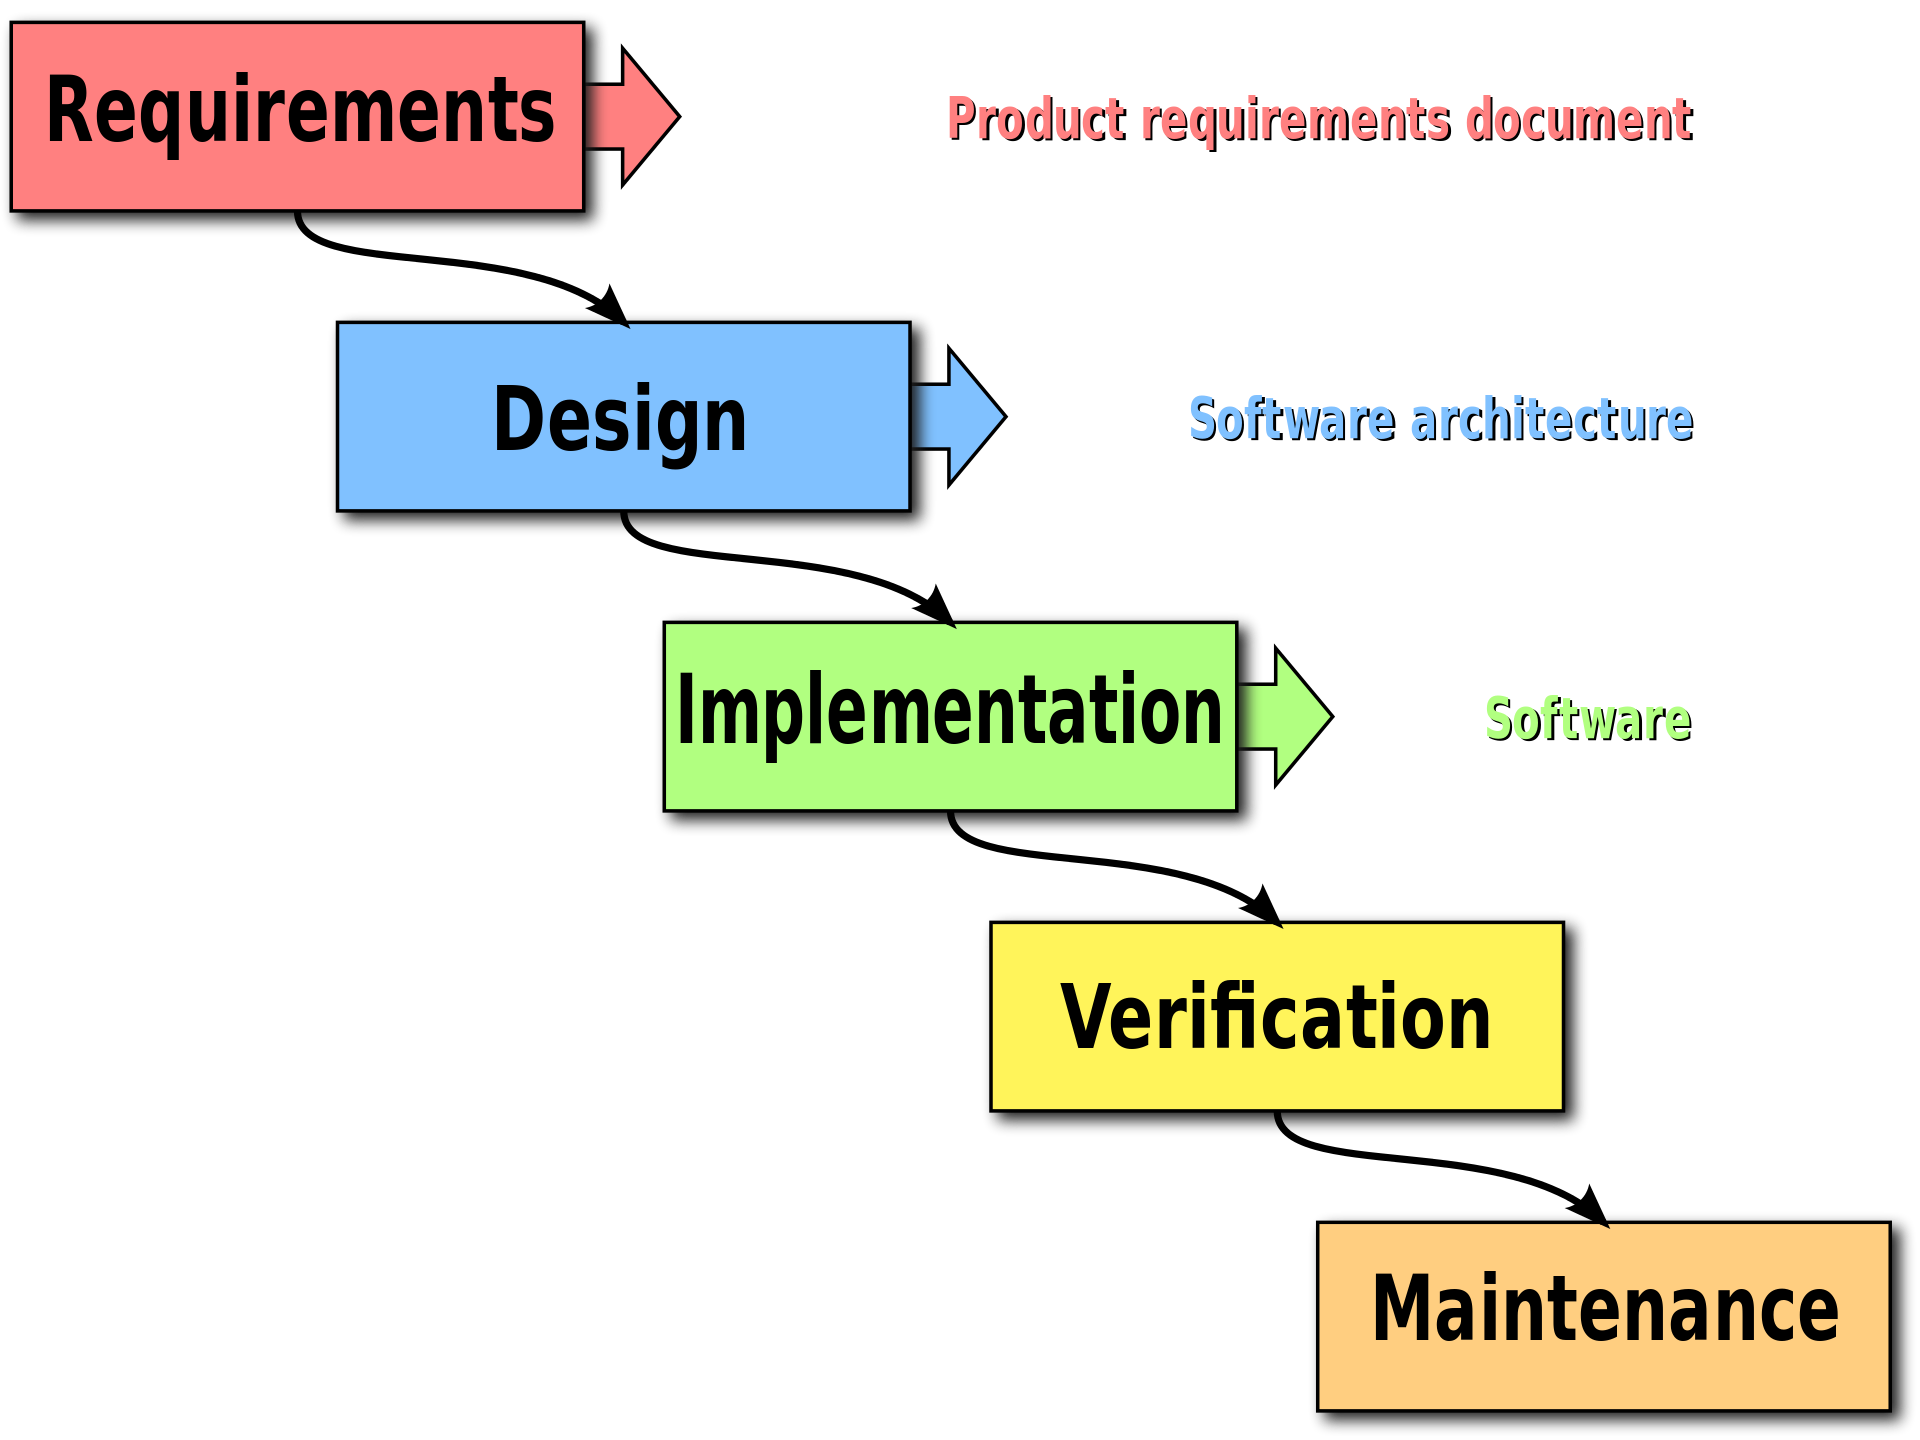
\includegraphics[width=0.8\linewidth]{lifecycle/img/waterfall}
\else
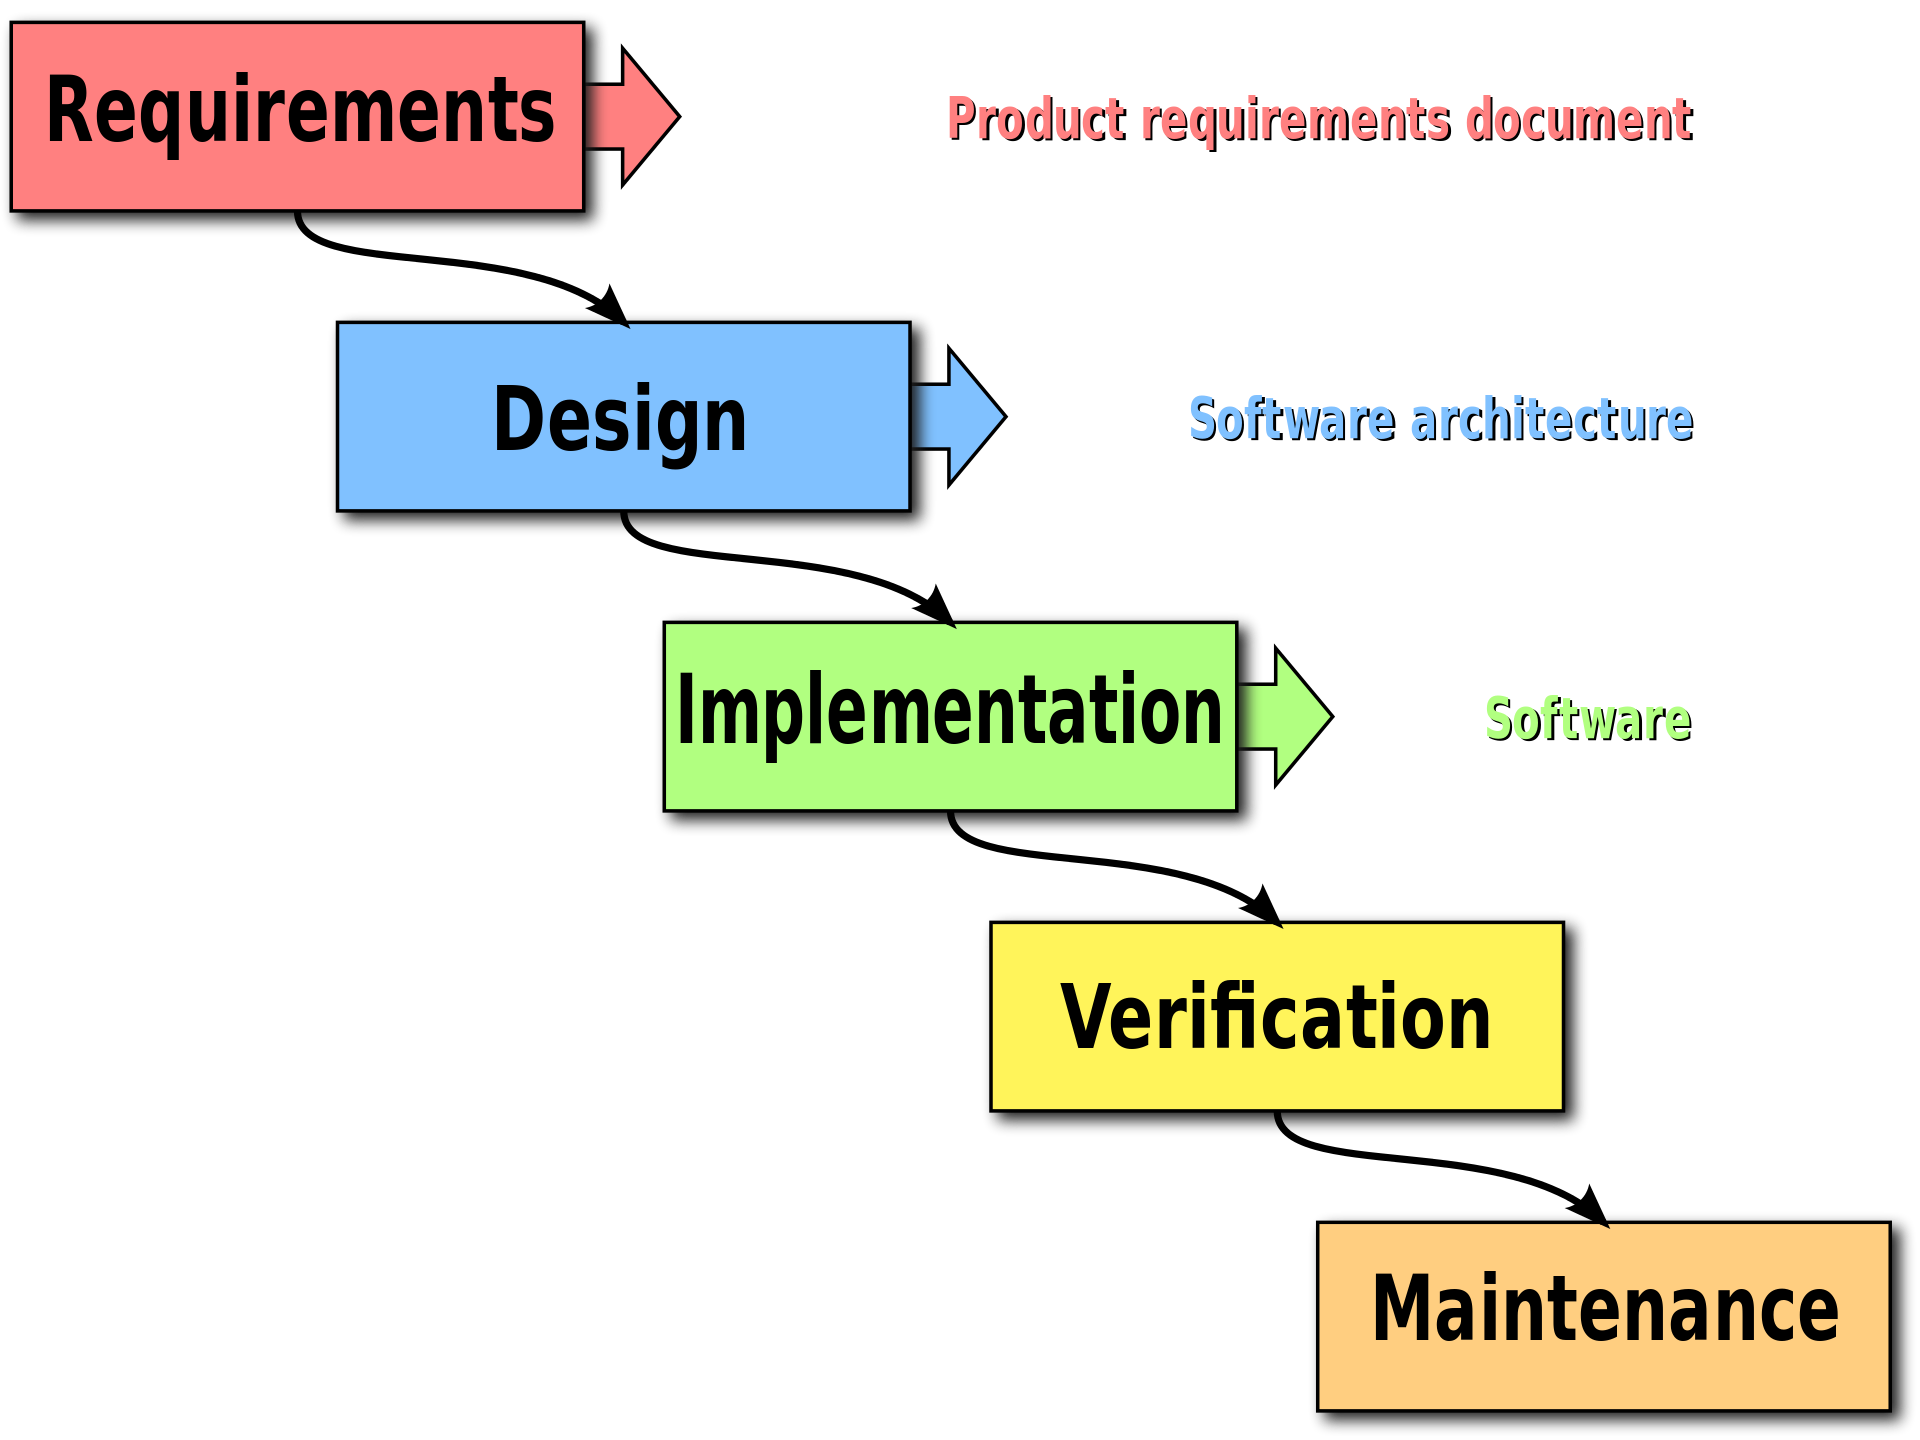
\includegraphics[width=0.8\linewidth]{lifecycle/img/waterfall}
\fi
\end{center}
\end{minipage}
\vspace{1cm}
\newpage
\section{Spiral model}
Risk driven, incremental
%zyklisch, risiko-orientiert
\begin{center}
%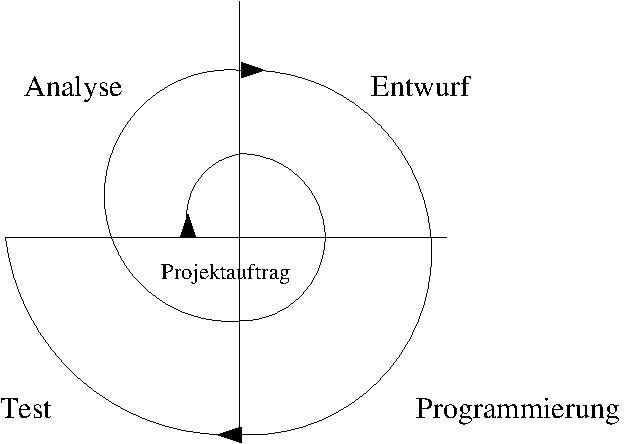
\includegraphics[width=0.6\linewidth]{lifecycle/xfig/spiral}
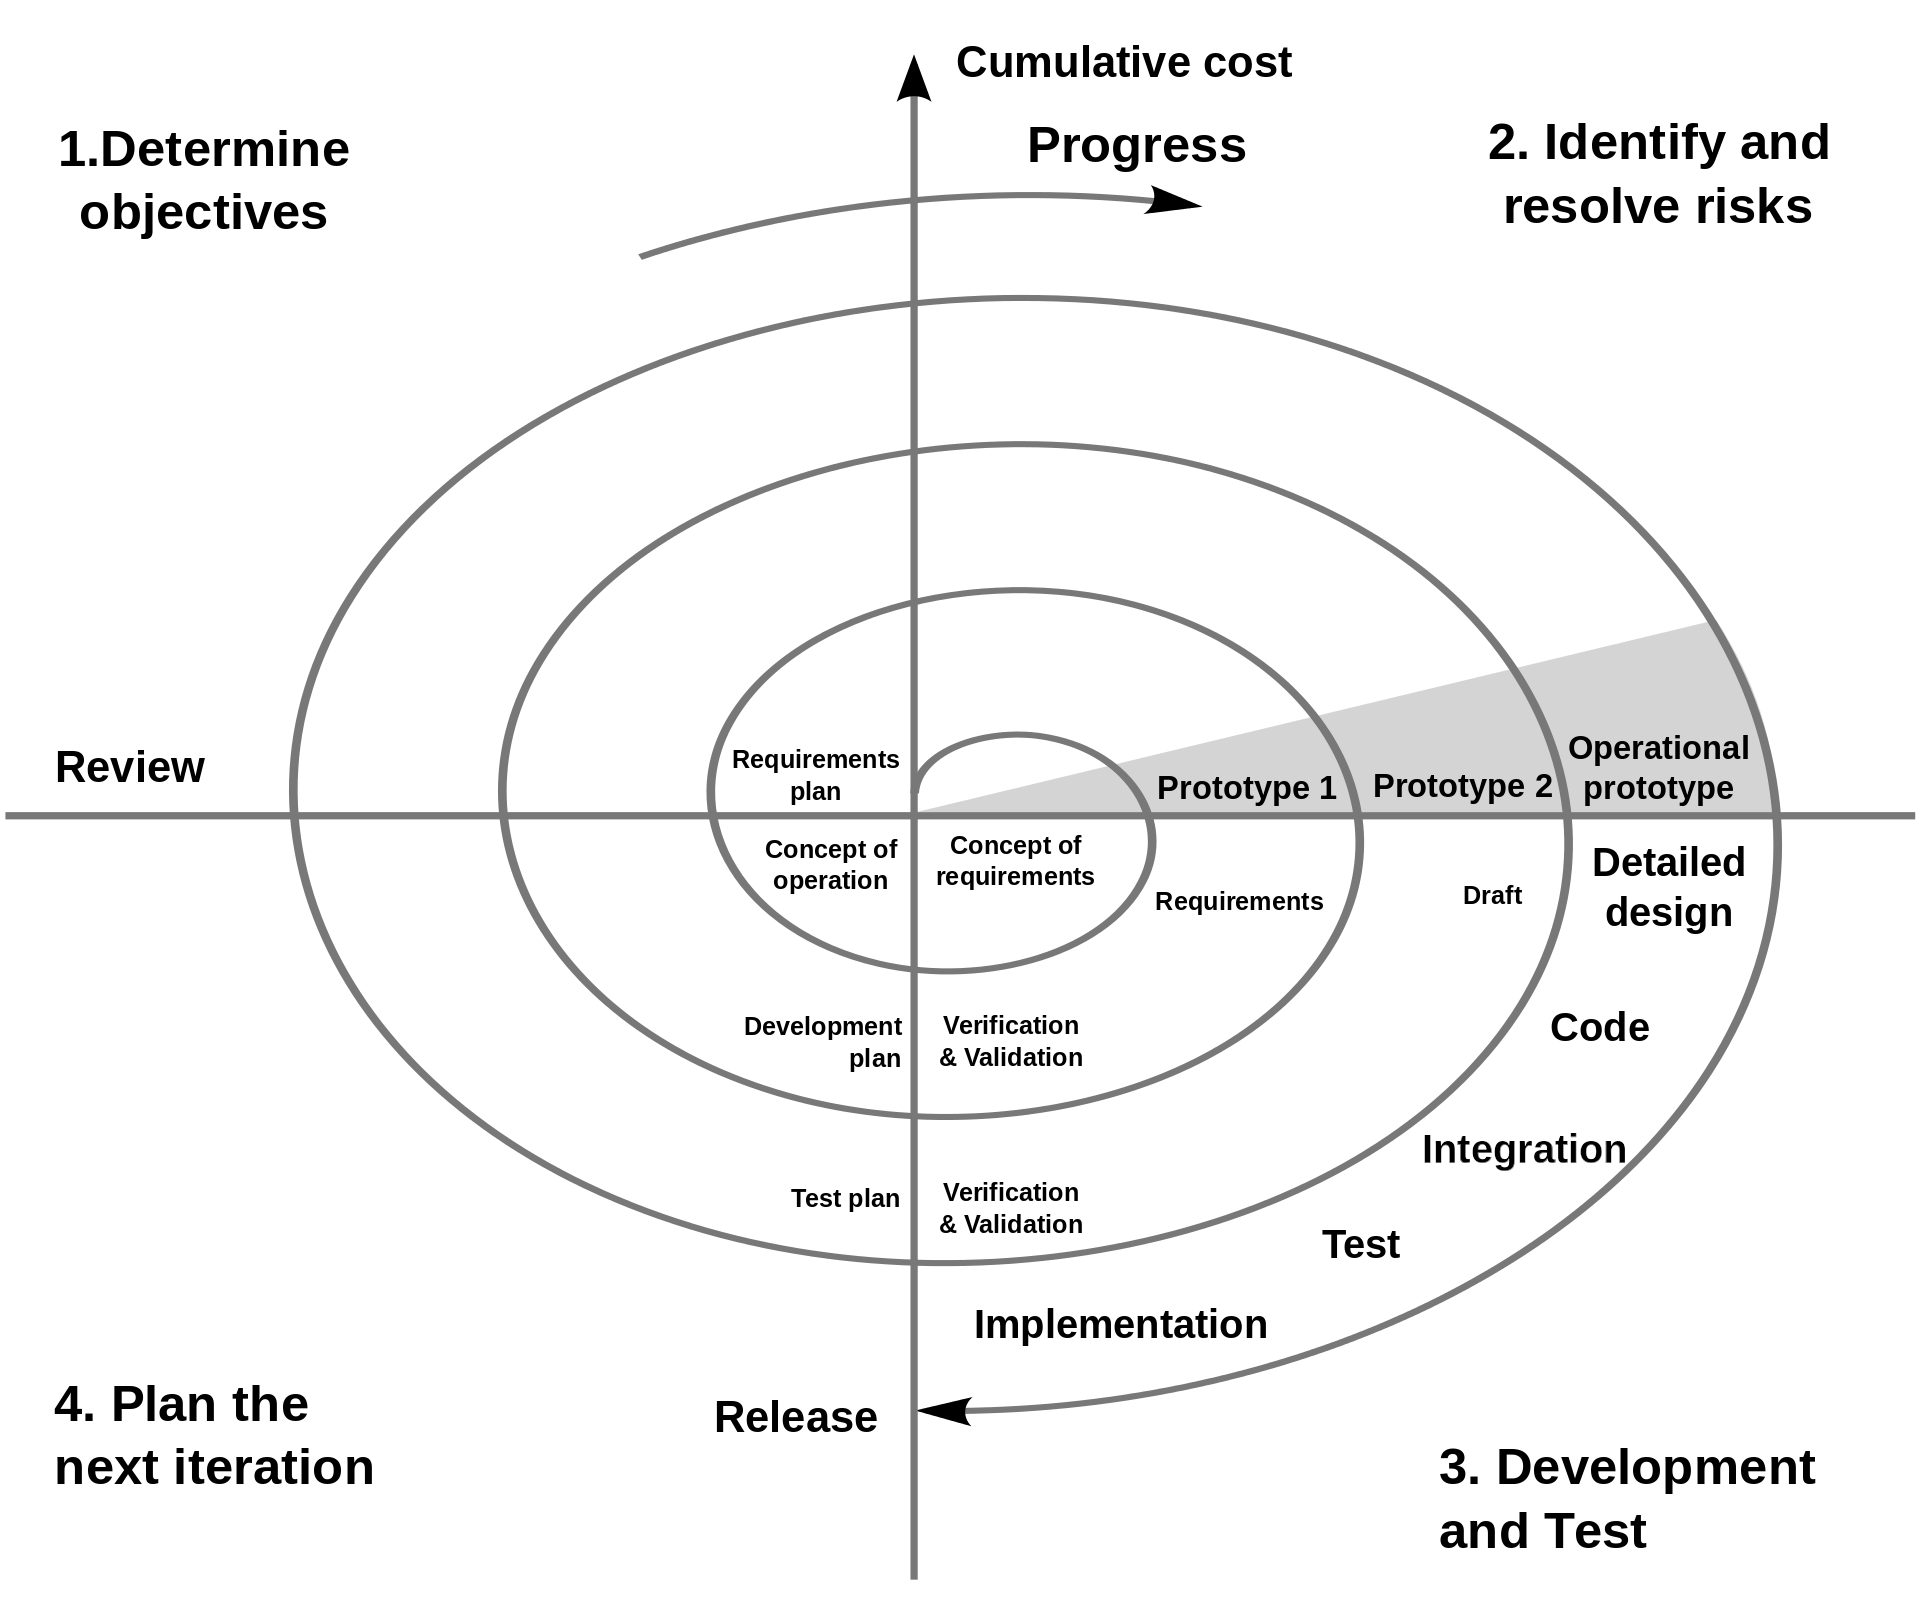
\includegraphics[width=0.6\linewidth]{lifecycle/img/spiralmodel}
\end{center}
%
\section{Hermes}
\ifslides
\else
%Ein offener Standard zur Führung und Abwicklung von Informatikprojekten
%in- und ausserhalb der schweizerischen Bundesverwaltung (seit 1975, letzte
%Überarbeitung/Aktualisierung 2003, neuste Version 5.1, 2014)
HERMES is the project management method for projects in the area of IT,
service and product development, and business organization adjustment.
HERMES supports the steering, management and execution of projects with various
levels of complexity and different features. As a method, HERMES has a clear,
easy-to-understand structure, has a modular design and can be expanded.
 \href{https://www.hermes.admin.ch}{www.hermes.admin.ch}
\begin{figure}[H]
\fi
\begin{center}
\ifslides
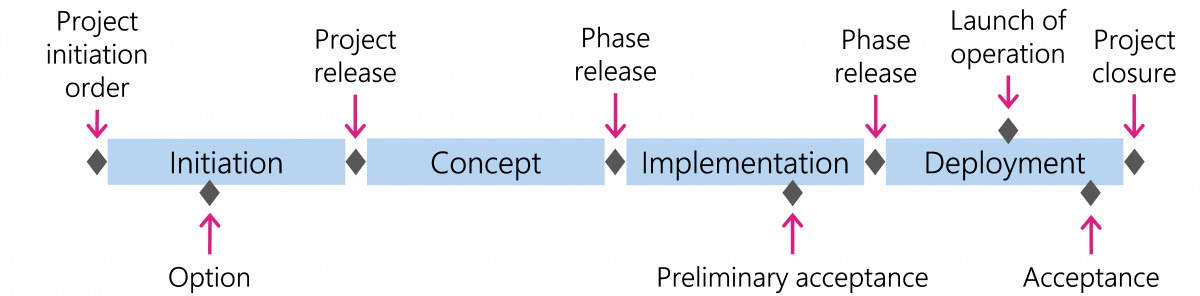
\includegraphics[width=\linewidth]{lifecycle/img/hermes}
\else
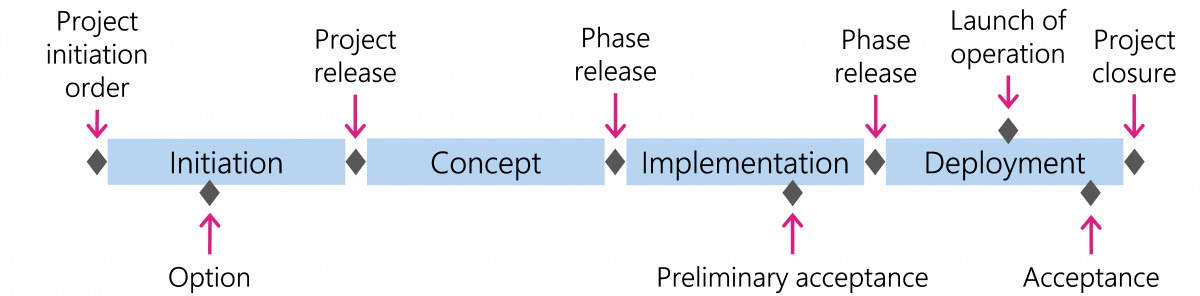
\includegraphics[width=\linewidth]{lifecycle/img/hermes}
\fi
%%\caption{Source: Informatikstrategieorgan des Bundes}
\end{center}
\ifslides
\else
\end{figure}
\fi
%\vspace{2cm}
The phase model forms the backbone of the project. It subdivides the life
cycle of the project and creates the conditions for the project participants
common understanding of the course of the project. The HERMES phase model
consists of four phases:
\begin{description}
\item[Initiation] During the initiation phase, the objectives are defined in
the study and the requirements are worked out in sufficient detail for options
to be developed and evaluated. The project order is created on the basis of the
option selected.
\item[Concept] In the concept phase, the rough requirements documented in the
study are fleshed out and completed as system requirements. Project-specific
solution concepts are designed in detailed studies. They form part of the system
architecture. This describes the system with its processes, functionality,
system components and their integration into the system environment via interfaces.
\item[Implementation] Based on the system architecture, the detailed
specifications are created and the system is developed according to those.
This also includes testing as a prerequisite for the decision on preliminary
acceptance.
\item[Deployment] In the deployment phase, the system is activated and then the
decision on acceptance is made.
\end{description}

\newslide

HERMES offers eight standard scenarios for projects with different characteristics:

\structure{Scenarios}: Anpassung an jeweilige Projektcharakteristiken:
\begin{itemize}
%\item IT-Individualanwendung: Entwicklung und Integration
%\item IT-Standardanwendung: Beschaffung und Integration
%\item IT-Anwendung-Weiterentwicklung
%\item IT-Infrastruktur: Erweiterung, Anpassung
%\item Dienstleistung/Produkt
%\item Organisationsanpassung

\item Service/product
\item Customized IT application
\item Standard IT application
\item Further development of IT application
\item IT infrastructure
\item Organizational adjustment
\item Service/product (agile)
\item Customized IT application (agile)
\end{itemize}

\structure{Modules}: wiederverwerwendbare Bausteine zur Erstellung von Szenarien
\begin{itemize}
%\item Beschaffung
%\item Einführungsorganisation
%\item Entwicklung
%\item Geschäftsorganisation
%\item Informationssicherheit und Datenschutz
%\item IT Betrieb, -Migration, -System
%\item Produkt
%\item Projektführung, -grundlagen, -steuerung
%\item Testen

\item Project steering
\item Project management
\item Agile development
\item Project foundations
\item Business organization
\item Product
\item IT system
\item Procurement
\item Deployment organization
\item Testing
\item IT migration
\item IT operation
\item Information security and data protection
\end{itemize}
Ergänzung: Marketing, Kommunikation, Personalentwicklung, Ausbildung, Strategieentwicklung, Einführung Geschäftsverwaltung
\newslide

\section{V-Modell}
The V-model is a graphical representation of a systems development
lifecycle. It is used to produce rigorous development lifecycle models
and project management models. The key attribute of using a
"V" representation was to require proof that the products from the left-side
of the V were acceptable by the appropriate test and integration
organization implementing the right-side of the V.\\

\vspace{3mm}

\begin{figure}[H]
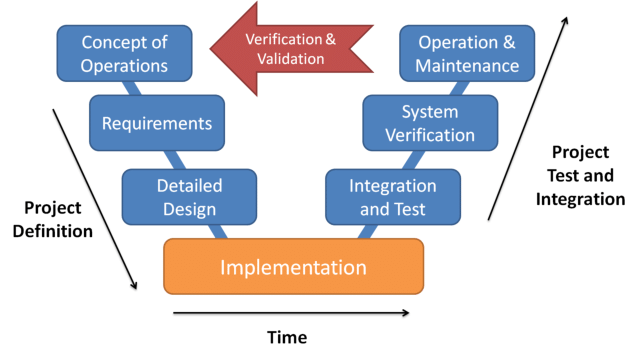
\includegraphics[width=\linewidth]{lifecycle/img/vmodell}
\end{figure}

\subsection{2 Streams}
There are two streams, one stream on each side of the V.
\begin{itemize}
\item Specification Stream\\
User Requirements Specification, Functional Requirement Specification, Design specification
\item Testing Stream\\
Installation qualification, Operational qualification, Performance qualification
\end{itemize}

\subsection{Advantages}
\begin{itemize}
\item The users of the V-model participate in the development and
maintenance of the V-model. A change control board publicly maintains
the V-Model. The change control board meets anywhere from every day to
weekly and processes all change requests received during system development
and test.
\item The V-model provides concrete assistance on how to implement an
activity and its work steps, defining explicitly the events needed to
complete a work step: each activity schema contains instructions,
recommendations and detailed explanations of the activity.
\end{itemize}

\newpage
\section{PRINCE2}
PRINCE2 is a project management method widely adopted around the world,
used by people and organizations from wide-ranging industries and sectors.

It is a flexible method that guides you through the essentials for
managing successful projects, regardless of type or scale. Built
upon seven principles, themes and processes, PRINCE2 can be tailored
to meet your specific requirements.

%1996
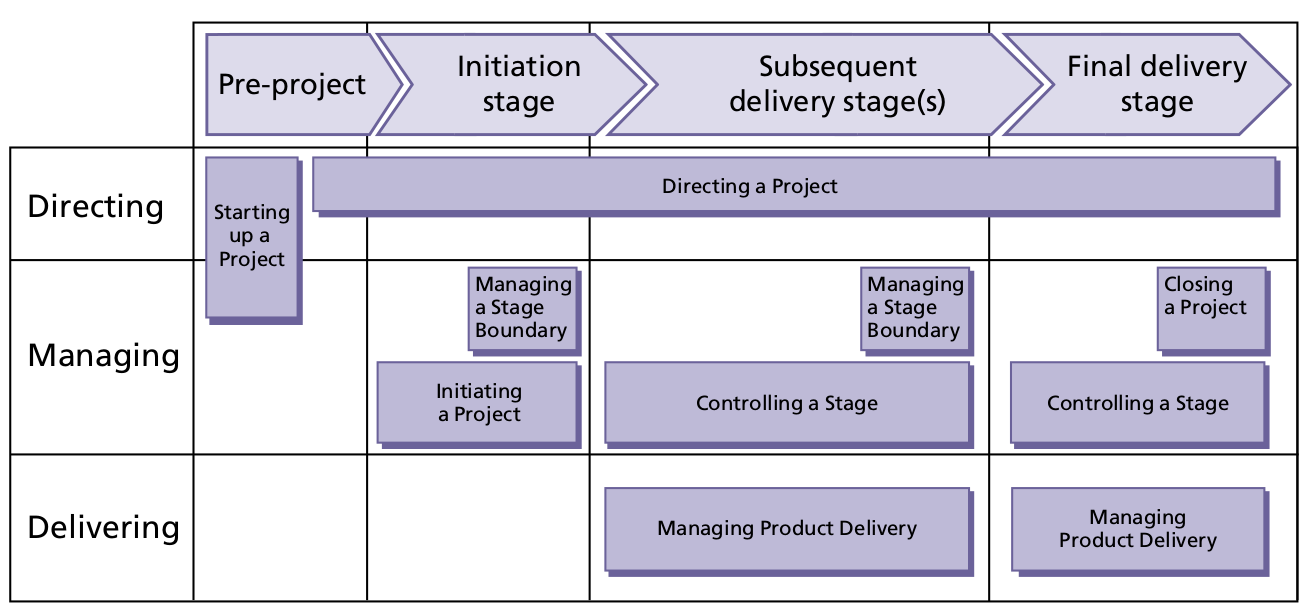
\includegraphics[width=\linewidth]{lifecycle/img/prince2}

\newslide
The Modell includes the following 8 processes:
  (\href{https://www.prince-officialsite.com}{www.prince-officialsite.com})
\begin{description}
\item [1. Directing a Project (DP)]:
Directing a Project runs from the start-up of the project until its
closure. This process is aimed at the Project Board. The Project Board manages
by exception, monitors via reports and controls through a number of decision
points.

The key processes for the Project Board break into four main areas:
\begin{itemize}
\item Initiation (starting the project off on the right foot)
\item Stage boundaries (commitment of more resources after checking results so
  far)
\item Ad hoc direction (monitoring progress, providing advice and guidance,
  reacting to exception situations)
\item Project closure (confirming the project outcome and controlled close).
\end{itemize}
This process does not cover the day-to-day activities of the Project Manager.
%
\ifslides
\newpage
\fi
\item [2. Starting up a Project (SU)]:
This is the first process in PRINCE. It is a pre-project process, designed to
ensure that the pre-requisites for initiating the project are in place. The
process expects the existence of a Project Mandate which defines in high level
terms the reason for the project and what outcome is sought. Starting up a
Project should be very short.

The work of the process is built around the production of three elements:
\begin{itemize}
\item Ensuring that the information required for the project team is available
\item Designing and appointing the Project Management Team
\item Creating the Initiation Stage Plan.
\end{itemize}
%
\ifslides
\newpage
\fi
\item[3. Initiating a Project (IP)]: The objectives of Initiating a Project are to:
  \begin{itemize}
  \item Agree whether or not there is sufficient justification to proceed with
  the project
\item Establish a stable management basis on which to proceed
\item Document and confirm that an acceptable Business Case exists for the
  project
\item Ensure a firm and accepted foundation to the project prior to
  commencement of the work
\item Agree to the commitment of resources for the first stage of the project
\item Enable and encourage the Project Board to take ownership of the project
\item Provide the baseline for the decision-making processes required during
  the project's life
\item Ensure that the investment of time and effort required by the project is
  made wisely, taking account of the risks to the project.
  \end{itemize}
\ifslides
\newpage
\fi
\item[4. Managing Stage Boundaries (SB)]:
This process provides the Project Board with key decision points on whether to
continue with the project or not. The objectives of the process are to:
\begin{itemize}
\item Assure the Project Board that all deliverables planned in the current
  Stage Plan have been completed as defined
\item Provide the information needed for the Project Board to assess the
  continuing viability of the project
\item Provide the Project Board with information needed to approve the current
  stage's completion and authorise the start of the next stage, together with
  its delegated tolerance level
\item Record any measurements or lessons which can help later stages of this
  project and/or other projects.
\end{itemize}
\ifslides
\newpage
\fi
\item [5. Controlling a Stage (CS)]:
This process describes the monitoring and control activities of the Project
Manager involved in ensuring that a stage stays on course and reacts to
unexpected events. The process forms the core of the Project Manager's effort
on the project, being the process which handles day-to-day management of the
project. Throughout a stage there will be a cycle consisting of:
\begin{itemize}
\item Authorising work to be done
\item Gathering progress information about that work
\item Watching for changes
\item Reviewing the situation
\item Reporting
\item Taking any necessary corrective action.
\end{itemize}
This process covers these activities, together with the on-going work of risk
management and change control.
\ifslides
\newpage
\fi
\item [6. Managing Product Delivery (MP)]:
The objective of this process is to ensure that planned products are created
and delivered by:
\begin{itemize}
\item Making certain that work on products allocated to the team is
  effectively authorised and agreed e accepting and checking Work Packages
\item Ensuring that work conforms to the requirements of interfaces identified
  in the Work Package
\item Ensuring that the work is done
\item Assessing work progress and forecasts regularly
\item Ensuring that completed products meet quality criteria
\item Obtaining approval for the completed products.
\end{itemize}
\ifslides
\newpage
\fi
\item [7. Closing a Project (CP)]:
The purpose of this process is to execute a controlled close to the
project. The process covers the Project Manager's work to wrap up the project
either at its end or at premature close. Most of the work is to prepare input
to the Project Board to obtain its confirmation that the project may close.

The objectives of Closing a Project are, therefore, to:
\begin{itemize}
\item Check the extent to which the objectives or aims set out in the Project
  Initiation Document (PID) have been met
\item Confirm the extent of the fulfilment of the Project Initiation Document
  (PID) and the Customer's satisfaction with the deliverables
\item Obtain formal acceptance of the deliverables
\item Ensure to what extent all expected products have been handed over and
  accepted by the Customer
\item Confirm that maintenance and operation arrangements are in place (where
  appropriate)
\item Make any recommendations for follow-on actions
\item Capture lessons resulting from the project and complete the Lessons
  Learned Report
\item Prepare an End Project Report
\item Notify the host organisation of the intention to disband the project
  organisation and resources.
\end{itemize}
\ifslides
\newpage
\fi
\item [8. Planning (PL)]
Planning is a repeatable process, and plays an important role in other
processes, main ones being:
\begin{itemize}
\item Planning an Initiation Stage (SL16)
\item Planning a Project (IP2)
\item Planning a Stage (SB1)
\item Producing an Exception Plan (SB6).
\end{itemize}
PRINCE provides a product-based start to the planning activity. It also provides planning framework which can be applied to any type of project. This involves:
\begin{itemize}
\item Establishing what products are needed
\item Determining the sequence in which each product should be produced
\item Defining the form and content of each product
\item Resolving what activities are necessary for their creation and delivery.
\end{itemize}
\end{description}
\ifslides
\newpage
\fi
Managers using PRINCE are able to...
\begin{itemize}
\item Establish terms of reference as a pre-requisite to the start of a
  project
\item Use a defined structure for delegation, authority and communication
\item Divide the project into manageable stages for more accurate planning
\item Ensure resource commitment from management is part of any approval to
  proceed
\item Provide regular but brief management reports
\item Keep meetings with management and stakeholders to a minimum but at the
  vital points in the project.
\end{itemize}
\ifslides
\newpage
\fi
Those who will be directly involved with using the results of a project are able to...
\begin{itemize}
\item Participate in all the decision-making on a project
\item If desired, be fully involved in day-to-day progress
\item Provide quality checks throughout the project and ensure their
\item requirements are being adequately satisfied.
\end{itemize}
For senior management PRINCE uses the 'management by exception' concept. They
are kept fully informed of the project status without having to attend
regular, time-consuming meetings.
\ifslides
\else
\newpage
\fi
\section{Unified-Process}
\ifslides
%Rational Corp (Ivar Jacobson)
\else
The Unified Process is not simply a process, but rather an extensible
framework which should be customized for specific organizations or
projects. The Rational Unified Process is, similarly, a customizable
framework. As a result, it is often impossible to say whether a
refinement of the process was derived from UP or from RUP, and so
the names tend to be used interchangeably.\\

The name Unified Process as opposed to Rational Unified Process is
generally used to describe the generic process, including those elements
which are common to most refinements. The Unified Process name is also
used to avoid potential issues of trademark infringement since Rational
Unified Process and RUP are trademarks of IBM.
\fi
\begin{center}
\ifslides
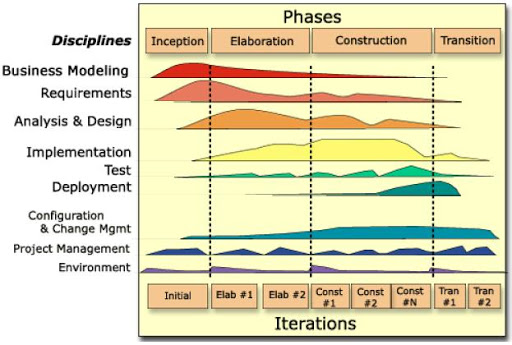
\includegraphics[width=0.8\linewidth]{lifecycle/img/unifiedprocess.jpg}
\else
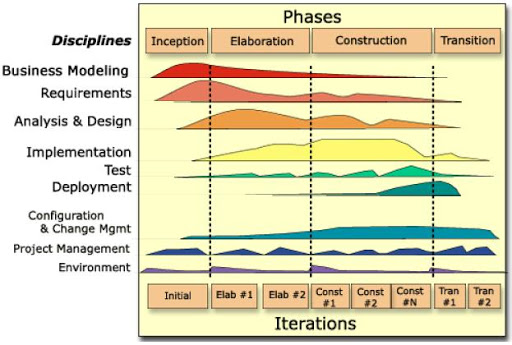
\includegraphics[width=0.9\linewidth]{lifecycle/img/unifiedprocess.jpg}
\fi
\end{center}
\vspace{1.5cm}

\begin{description}
\item[Use-Case-Driven]:\\
  Use case driven means that use cases are used as a primary artifact for
  establishing the desired behavior of the system, for verifying and
  validating the system's architecture, for testing, and for communicating
  among the stakeholders of the project.
\item[Architecture-centric]:\\
  Architecture-centric means that a system's architecture is used as a
  primary artifact for conceptualizing, constructing, managing, and
  evolving the system under development.
\item[Iterative and incremental]:\\
  An iterative process is one that involves managing a stream of
  executable releases. An incremental process is one that involves
  the continuous integration of the system's architecture to produce
  these releases, with each new release embodying incremental improvements
  over the other. Together, an iterative and incremental process is
  risk-driven, meaning that each new release is focused on attacking and
  reducing the most significant risks to the success of the project.
\end{description}
\newpage
\subsection{Phases}
\begin{description}
\item[Inception]:\\
  The idea for the project is stated. The development team determines
  if the project is worth pursuing and what resources will be needed.
\item[Elaboration]:\\
  The project's architecture and required resources are further evaluated.
  Developers consider possible applications of the software and costs
  associated with the development.
\item[Construction]:\\
  The project is developed and completed. The software is designed,
  written, and tested.
\item[Transition]:\\
 The software is released to the public. Final adjustments or updates are
 made based on feedback from end users.
 The Transition phase also includes system conversions and user training.
\end{description}

\subsection{Workflows}
\begin{description}
\item[Business Modelling]:\\
  During this workflow, the business context (scope) of the project should be
  outlined.
\item[Requirements]:\\
  Used to define all potential requirements of the project, throughout the
  software development life cycle.
\item[Analysis and Design]:\\
  Once the requirements workflow is complete, the analysis and design phase
  takes those requirements and transforms them into a design that can be
  properly implemented.
\item[Implementation]:\\
  This is where the majority of actual coding takes place, implementing and
  organizing all the code into layers that make up the whole of the system.
\item[Test]:\\
  Testing of all kinds takes place within this workflow.
\item[Deployment]:\\
  Finally, the deployment workflow constitutes the entire delivery and
  release process, ensuring that the software reaches the customer as expected.
\item[Configuration Management]:\\
Used to describe the various artifacts produced by the development team,
ideally ensuring that there is minimal overlap or wasted efforts performing
similar activities that result in identical or conflicting artifacts.
\item[Project Management]:\\
Where all activities dealing with project management take place, from pushing
design objectives to managing risk to overcoming delivery constraints.
\item[Environment]:\\
Finally, this workflow handles the setup and management of all software
development environments throughout the team, including the processes,
as well as the tools, that are to be used throughout the software
development life cycle.

\end{description}
%%
\newpage
\section{Extreme Programming (XP)}
Extreme programming (XP) is a software development methodology which is
intended to improve software quality and responsiveness to changing customer
requirements. As a type of agile software development,
it advocates frequent "releases" in short development cycles, which is
intended to improve productivity and introduce checkpoints at which new
customer requirements can be adopted. \href{https://www.extremeprogramming.org}
{www.extremeprogramming.org}
\begin{center}
\ifslides
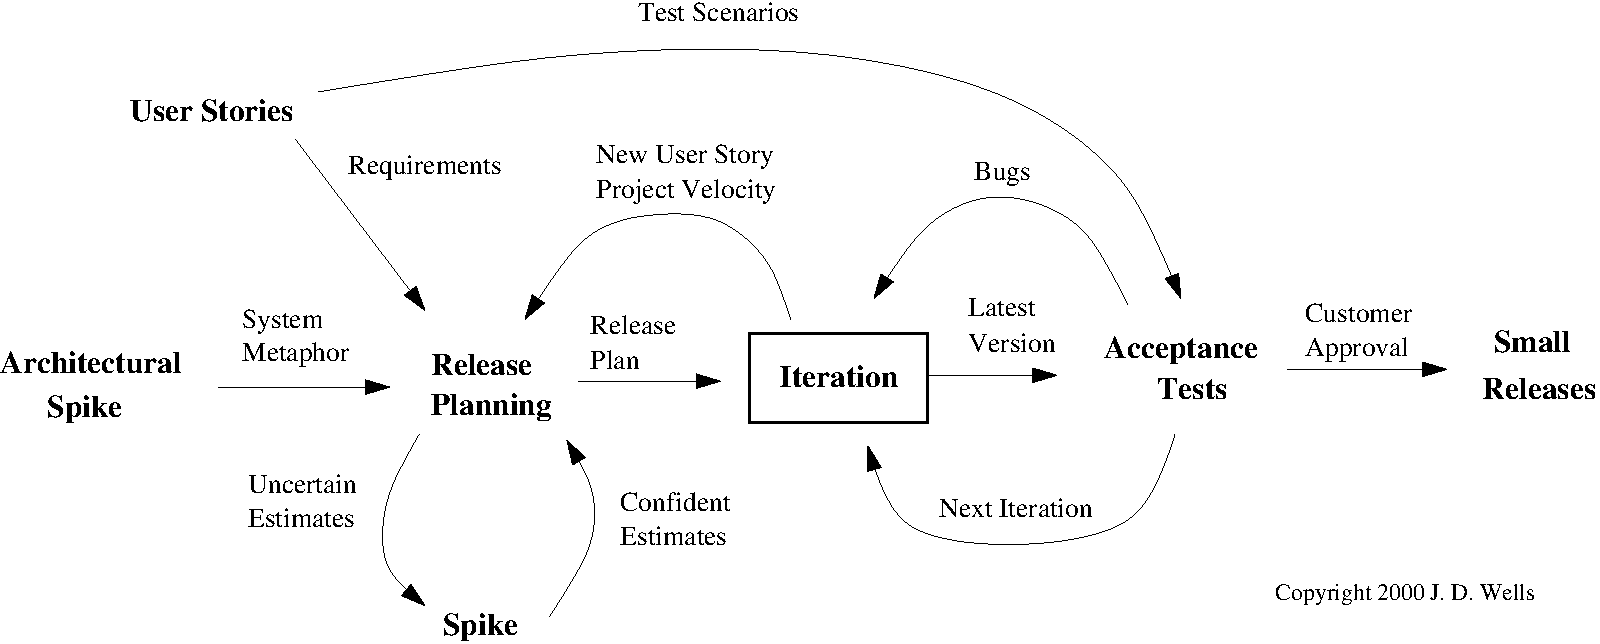
\includegraphics[width=0.9\linewidth]{lifecycle/xfig/xp-project}
\else
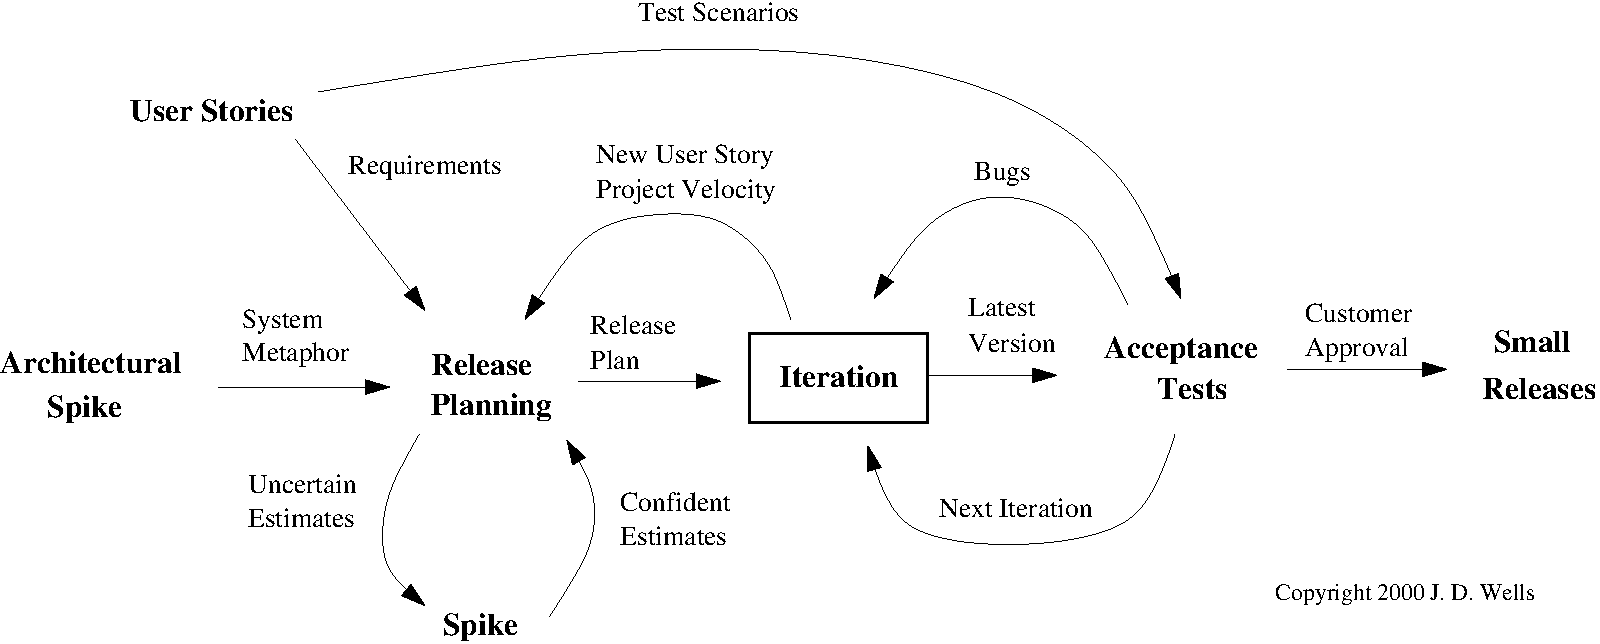
\includegraphics[width=0.8\linewidth]{lifecycle/xfig/xp-project}
\fi
\end{center}
%\section*{Extreme-Programming Grundsätze}

\subsection{Values}
Extreme Programming has simple rules that are based on 5 values:

\begin{description}
\item [Communication]:\\
Everyone on a team works jointly at every stage of the project.
\item  [Simplicity]:\\
Developers strive to write simple code bringing more value to a product, as it
saves time and efforts.
\item [Feedback]:\\
Team members deliver software frequently, get feedback about it, and improve a
product according to the new requirements.
\item [Respect]:\\
Every person assigned to a project contributes to a common goal.
\item [Courage]:\\
Programmers objectively evaluate their own results without making excuses and
are always ready to respond to changes.
\end{description}


\subsection{Principles}
Most researches link XP with the following 5 principles:

\begin{description}
\item [Rapid feedback]:\\
Team members understand the given feedback and react to it right away.
\item [Assumed simplicity]:\\
Developers need to focus on the job that is important at the moment and
follow YAGNI (You Ain't Gonna Need It) and DRY (Don't Repeat Yourself)
principles.
\item [Incremental changes]:\\
Small changes made to a product step by step work better than big ones made at
once.
\item [Embracing change]:\\
If a client thinks a product needs to be changed, programmers should support
this decision and plan how to implement new requirements.
\item [Quality work]:\\
A team that works well, makes a valuable product and feels proud of it.
\end{description}


\subsection{12 Practices}
XP suggests using 12 practices while developing software.

\begin{description}
\item [Test-Driven Development]:
\item [The Planning Game]:
\item [On-site Customer]:
\item [Pair Programming]:
\item [Code Refactoring]
\item [Continuous Integration]
\item [Small Releases]
\item [Simple Design]
\item [Coding Standards]
\item [Collective Code Ownership]
\item [System Metaphor]
\item [Work Condition]
\end{description}
%
\newpage
\subsection{User Story vs Use Case}
A \textbf{user story} is a short description of something that your customer will
do when they come to your website or use your application/software,
focused on the value or result they get from doing this thing. They are
written from the point of view of a person using your website or application,
and written in the language that your customers would use.\\

\newslide
Examples (\href{https://www.agilemodeling.com/artifacts/userStory.htm}
     {www.agilemodeling.com/artifacts/userStory.htm}):
\begin{itemize}
\item Students can purchase monthly parking passes online.
\item Parking passes can be paid via credit cards.
\item Parking passes can be paid via PayPal ™.
\item Professors can input student marks.
\item Students can obtain their current seminar schedule.
\item Students can order official transcripts.
\item Students can only enroll in seminars for which they have prerequisites.
\item Transcripts will be available online via a standard browser.
\end{itemize}

A \textbf{user story} is usually written using the format canonised by Mike Cohn:
\emph{As an [actor] I want [action] so that [achievement]}.\\
So, for example: \emph{As a Flickr member, I want to set different privacy levels
on my photos, so I can control who sees which of my photos}.\\


A \textbf{use case} is a description of a set of interactions between a
system and and one or more actors (where actor can be people, or other
systems: for example, both online shoppers and PayPal can be actors).
They are usually created as documents, and generally include this kind
of information:

\ifslides
\else
\begin{tabularx}{\linewidth}{lX}
%\begin{tabular}{|l|l|}
  \toprule % booktabs package
  Title & Name of use case \\
  \midrule
    Description & some short text describing the scope.\\
  \midrule
    Actor(s) & person(s) who interact with this particular use case. \\
  \midrule
    Precondition & anything that this use case can assume to be true
                        prior to beginning it's life cycle.\\
  \midrule
    Success scenario & a sequence of steps describing correct flow of
         events that take place.\\
  \midrule
  Extensions & flow of application when it deviates from success scenario's flow:
    \begin{itemize}
    \item
      Alternate flows - other options of correct flow
    \item
      Exception flows - flow of events for when things go wrong
    \end{itemize}\\
  \midrule
        Post condition &  state of application after everything is done\\
        \bottomrule
\end{tabularx}\\[2ex]
\fi

%
\subsection{INVEST (Bill Wake)}
\begin{tabularx}{\linewidth}{l|l|X}
  I & Independent &The user story should be self-contained, in a way that there is no inherent dependency on another user story. \\
  N & Negotiable & User stories, up until they are part of an iteration, can always be changed and rewritten.\\
  V & Valuable & A user story must deliver value to the end user.\\
  E & Estimable & You must always be able to estimate the size of a user story.\\
  S & Small & User stories should not be so big as to become impossible to plan/task/prioritize with a certain level of certainty.\\
  T & Testable & The user story or its related description must provide the necessary information to make test development possible.\\
\end{tabularx}
\newpage
\section{Scrum}
Scrum (Rugby: Gedränge) ist ein agiles Vorgehensmodell für die
Entwicklung komplexer Softwaresysteme. Ursprünglich von Hirotaka
Takeuchi und Ikujiro Nonaka beschrieben, wurde es einige Jahre später von
Jeff Sutherland und Ken Schwaber in Firmen eingesetzt und als Referenz
an ein Rugby-Team

.. tries to go to the distance as a unit, passing the ball back and forth

Scrum genannt.

\newslide
Der Scrum-Prozess beginnt mit der Zusammenstellung der Anforderungen
in Form von User Stories,
was hier als ``Product Backlog'' bezeichnet wird. Für die
Implementierung wählt das Team, welches üblicherweise aus 5-9
Entwicklern besteht, gemeinsam mit dem Kunden (dem Product
Owner) einen Satz von Anforderungen aus, die für die nächste Iteration
wichtig und sinnvoll sind. Dieser Satz wird ``Sprint Backlog''
genannt.
Er wird
getrennt vom Product Backlog verwaltet, da sich während einer
Iteration die Anforderungen ändern können. Dadurch entsteht eine
 Verbindlichkeit: die Entwickler lernen Aufwände besser zu
schätzen und Zusagen einzuhalten und die Kunden konkrete und
relevante Anforderungen zu stellen.
\begin{figure}[H]
\begin{center}
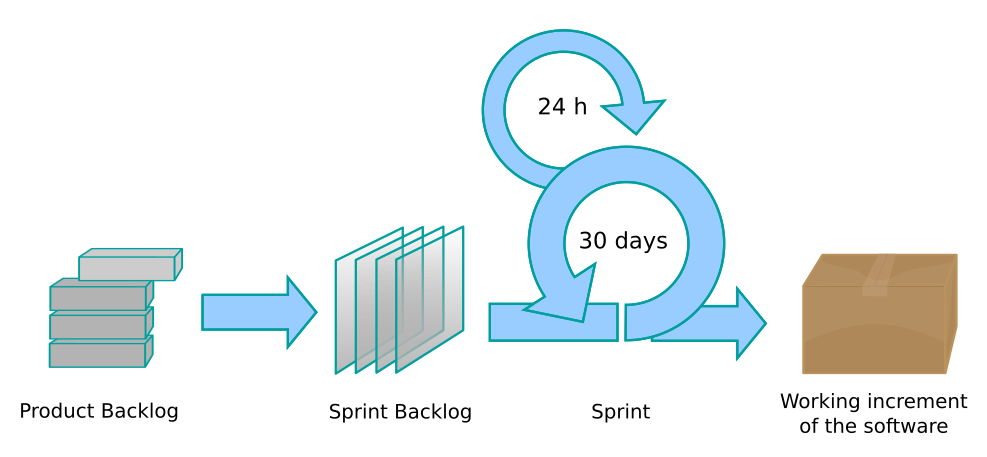
\includegraphics[width=\linewidth]{lifecycle/img/scrum_process}
\caption{Der Scrum-Prozess (Source: Wikipedia)}
\end{center}
\end{figure}
Ein Sprint dauert in der Regel etwa 15 - 30 Tage. Nach dieser Periode
sollte jeweils ein ausführbarer Release zur Verfügung stehen.

Zu Beginn eines Sprints werden die ausgewählten User Stories
in ein mehrspaltiges Taskboard (Sprint Backlog)
übertragen und in einzelne Tasks aufgeteilt:
Design, Implementierung, Test und Dokumentation. Die Tasks werden
in die Spalte ``zu erledigen'' (To Do) platziert. Im Laufe des Sprints
werden die einzelnen Tasks abgearbeitet, wobei die jeweilige Karte in
die entsprechende Spalte verschoben wird, um so den Projektfortschritt
zu dokumentieren.
\begin{figure}[H]
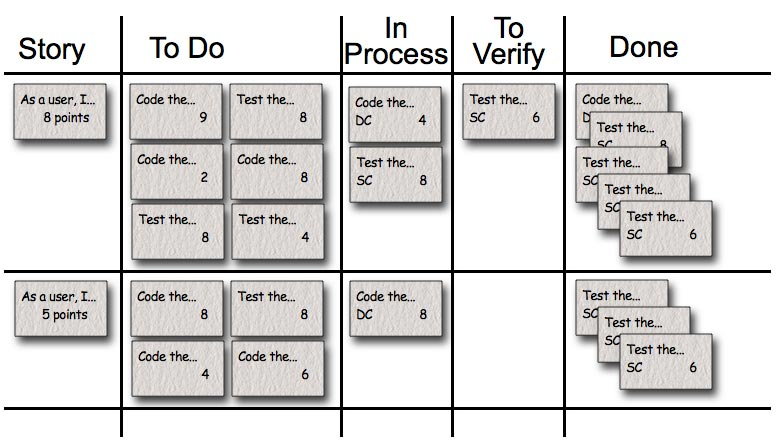
\includegraphics[width=\linewidth]{lifecycle/img/MockedTaskBoard}
\caption{Ein Scrum Taskboard (Source: www.mountaingoatsoftware.com)}
\end{figure}
%\newslide
Die Teilnehmer eines Scrum-Projektes werden in Pigs und Chicken
eingeteilt:
\begin{figure}[H]
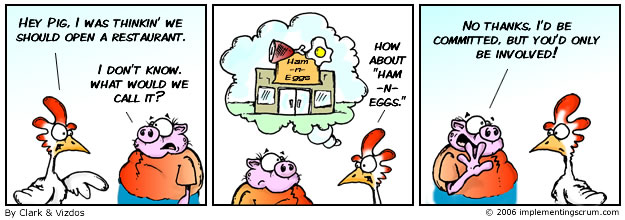
\includegraphics[width=\linewidth]{lifecycle/img/060911-scrumtoon}
\caption{Pigs und Chicken (Source: www.implementingscrum.com)}
\end{figure}
Als Pigs bezeichnet man Teilnehmer, die konkrete Verpflichtungen eingehen
(commit), während Chicken weniger direkt involvierte Teilnehmer sind
(User, Kunden, Anbieter, Manager \ldots).

In täglich durchgeführten Besprechungen (Daily Scrum) wird der
Kontext des aktuellen Tages festgelegt. Alle sind eingeladen daran
teilzunehmen aber nur ``Pigs'' dürfen sich äussern. Dabei geht
es im wesentlichen um die Fragen:
\begin{enumerate}
\item What did you do yesterday?
\item What will you do today?
\item Are there any impediments in your way?
\end{enumerate}
\newslide
Als typische Hindernisse (impediments) können auftreten:
\begin{itemize}
\item My \ldots broke and I need a new one today.
\item I still haven't got the software I ordered a month ago.
\item I need help debugging a problem with \ldots.
\item I'm struggling to learn \ldots and would like to pair with someone on it.
\item I can't get the vendor's tech support group to call me back.
\item Our new contractor can't start because no one is here to sign her contract.
\item I can't get the \ldots group to give me any time and I need to meet with them.
\item The department VP has asked me to work on something else "for a day or two."
\end{itemize}
Ein zuvor bestimmtes Team-Mitglied, der Scrum Master, sorgt dafür, dass
die Hindernisse so schnell wie möglich aus dem Weg geräumt werden.
%
\newslide
Weitere Informationen:
\begin{itemize}
\item Scrum: \href{https://www.scrumguides.org/scrum-guide.html}{www.scrumguides.org}
\item Eine Einführung: \href{https://mountaingoatsoftware.com/scrum}
    {mountaingoatsoftware.com/scrum}
\item Verschiedene Artikel
  \href{https://www.infoq.com/Agile}{www.infoq.com/Agile}
\item Scrum and XP from the Trenches (Henrik Kniberg)

  \href{https://www.infoq.com/minibooks/scrum-xp-from-the-trenches}
   {www.crisp.se/henrik.kniberg/ScrumAndXpFromTheTrenches.pdf}
%\item Beispiele:
%  \href{https://groups.google.com/group/allaboutagile/files}
%            {groups.google.com/group/allaboutagile/files}
%
\end{itemize}
%
\newpage
\section{The Cathedral and the Basar}
Eric Steven Raymond (ESR), US-amerikanischer Autor, Programmierer,
Mitgründer der OpenSource-Initiative hat 1997 ein Essay mit dem Titel
``The Cathedral and the Bazaar'' verfasst und am Linux-Kongress in
Würzburg präsentiert.

Er beschreibt darin die beiden unterschiedlichen Vorgehensmodelle
\begin{itemize}
\item \structure{Kathedrale}: ein zentralisierterer Ansatz mit sehr genauer
  Vorausplanung, gebaut wie Kathedralen, sorgsam gemeißelt von
  einzelnen Druiden oder kleinen Teams von Hohepriestern, die in
  totaler Abgeschiedenheit wirken und keine unfertigen Beta-Freigaben
  veröffentlichen dürfen.
\item \structure{Basar}: gekennzeichnet durch frühe und häufige Freigaben, dem
  Delegieren von allem, was nur irgendwie möglich ist, und der an
  Promiskuität grenzenden Offenheit - ein großer, wild durcheinander
  plappernder Basar von verschiedenen Zielsetzungen und Ansätzen,
  bei dem jeder etwas dazu beitragen kann.
\end{itemize}
\newslide
Voraussetzungen für Basar-Projekte:
\begin{itemize}
\item Basar-Projekte können nicht von Null an begonnen werden, man
benötigt ein herzeigbares, überzeugendes Versprechen (a plausible
promise).
Das Programm
braucht nicht besonders gut zu funktionieren. Es kann sehr
ungeschliffen, von Bugs geplagt, unvollständig und spärlich
dokumentiert sein. Was es aber nicht verfehlen darf, ist, (a) zu
laufen, und (b) potentielle Mit-Entwickler davon zu überzeugen, daß es
sich in absehbarer Zukunft zu etwas wirklich Tollem transformieren
läßt.
\item Der Koordinator oder Leiter eines Basar-Projekts muß mit Leuten
  umgehen und kommunizieren können. Um eine Entwicklergemeinde
  aufzubauen, muß man Menschen begeistern und für seine Sache
  interessieren können und bewirken, daß sie mit dem eigenen Anteil am
  Aufwand zufrieden sind.
\end{itemize}
%
\newpage
\section{Manifesto for Agile Software Development}
We are uncovering better ways of developing
software by doing it and helping others do it.
Through this work we have come to value:
\begin{description}
\item[Individuals and interactions] over processes and tools
\item[Working software] over comprehensive documentation
\item[Customer collaboration] over contract negotiation
\item[Responding to change] over following a plan
\end{description}
That is, while there is value in the items on
the right, we value the items on the left more.\\[2ex]
\begin{minipage}{0.3\linewidth}
Kent Beck\\
Mike Beedle\\
Arie van Bennekum\\
Alistair Cockburn\\
Ward Cunningham\\
Martin Fowler
\end{minipage}
\begin{minipage}{0.3\linewidth}
James Grenning\\
Jim Highsmith\\
Andrew Hunt\\
Ron Jeffries\\
Jon Kern\\
Brian Marick\\
\end{minipage}
\begin{minipage}{0.3\linewidth}
Robert C. Martin\\
Steve Mellor\\
Ken Schwaber\\
Jeff Sutherland\\
Dave Thomas\\
\end{minipage}\\[2ex]
\href{https://agilemanifesto.org}{agilemanifesto.org}

\newslide
\subsection{Manifesto for Software Craftmanship}

As aspiring Software Craftsmen we are raising the bar of professional software development
by practicing it and helping others learn the craft. Through this work we have come to value:
\begin{description}
\item[Not only working software] but also well-crafted software
\item[Not only responding to change] but also steadily adding value
\item[Not only individuals and interactions] but also a community of professionals
\item[Not only customer collaboration] but also productive partnerships
\end{description}

That is, in pursuit of the items on the left we have found the items on
the right to be indispensable.
\href{http://manifesto.softwarecraftsmanship.org}{manifesto.softwarecraftsmanship.org}

\newslide
Agil bedeutet wendig, flink:
\begin{itemize}
\item Die agilen Vorgehensmodelle betrachten
 die laufende Änderung der Anforderungen als ein \structure{natürlicher,
 unvermeidbarer} und \structure{wünschbarer Aspekt}.
\item Die Fähigkeit sich daran anzupassen ist \structure{realistischer} und
\structure{erfolgsversprechender}, als das Bestreben die Anforderungen
  bei Projektbeginn vollständig festzulegen.
\end{itemize}
Zitat Kent Beck (Extreme Programming explained):
\begin{quote}\em
Listening, Testing, Coding, Designing. That's all there is to
 software. Anyone who tells you different is selling something.
\end{quote}
